\documentclass[11pt]{article}
\usepackage[margin=1in]{geometry}
\usepackage[T1]{fontenc}
\usepackage{lmodern}
\usepackage{amsmath,amssymb,booktabs,array,graphicx}
\usepackage{hyperref}
\setlength{\emergencystretch}{8em}
\renewcommand{\arraystretch}{1.3}
\makeatletter
\newcommand{\sha}{\begingroup\catcode`\_=12 \sha@read}
\newcommand{\sha@read}[1]{\ttfamily\sha@loop#1\relax\endgroup}
\def\sha@loop#1{%
  \ifx\relax#1\else
    #1\allowbreak
    \expandafter\sha@loop
  \fi}
\makeatother
\hypersetup{colorlinks=true,linkcolor=blue,urlcolor=blue,citecolor=blue,
  pdftitle={Replication of the creative self-efficacy measurement models in Abbott (2010)},
  pdfauthor={}}
\newcommand{\abbottbase}{https://github.com/alectionary/vibe-math/blob/master/formalization/abbott-ctse}
\newcommand{\src}[1]{\href{\abbottbase/\detokenize{#1}}{\texttt{\detokenize{#1}}}}
\newcommand{\srcat}[2]{\href{\abbottbase/\detokenize{#1}\#L#2}{\texttt{\detokenize{#1}}}}

\title{Replication of the creative self-efficacy\\
measurement models in Abbott (2010)}
\author{}
\date{29 October 2026}

\begin{document}
\maketitle

\begin{abstract}
Does the revised measurement model for the Creative Thinking
Self-Efficacy inventory (CTSE~II) and the Creative Performance
Self-Efficacy inventory (CPSE~II) reproduce the sample correlations,
pass the printed fit cuts, and fit more parsimoniously than the rival
models?
Abbott (2010) answers yes.
The refined model has \(\chi^2(178)=295.571\),
\(\mathrm{CFI}=.954\), \(\mathrm{RMSEA}=.046\), and
\(\mathrm{SRMR}=.057\), and a lower Akaike information criterion than
the rival models.
CTSE and CPSE correlate with openness to experience and with Beghetto's
three-item creative self-efficacy measure.
A general factor does not improve the model.
We rebuilt the covariance matrix from the printed correlation matrix
and refit the Appendix~J models by maximum likelihood.
Every model has the printed degrees of freedom.
The standardized root mean square residual matches to about one
thousandth.
The implied-structure chi-square matches the maximum-likelihood value
implied by the printed scaled chi-square and its scaling factor,
\(715.13\) against \(714.98\).
The revised model remains the most parsimonious, and its Akaike gap
against the model that uses every indicator is \(234.12\) against the
printed \(235.09\).
The robust chi-square, comparative fit index, and root mean square
error of approximation of the revised model are not recovered from the
printed matrix.
The interview phase is not a covariance model and is not refit.
\end{abstract}

\section{The question, and the headline}
\label{sec:headline}

This section answers whether the printed measurement model is the one
in Appendix~J, and whether its fit statistics and its rank against the
rival models come back from the printed correlation matrix.
The degrees of freedom and the parsimony order do.
The standardized residual index does, to about one thousandth.
The robust chi-square and the two indices that are computed from it do
not, on this matrix.

Abbott (2010),
\url{https://digitalcommons.unl.edu/cehsdiss/68/},
asks how creative self-efficacy is structured.
Creative thinking self-efficacy has four factors: fluency, flexibility,
elaboration, and originality.
Creative performance self-efficacy has three: domain, field, and
personality.
The quantitative phase fits that model, a general-factor restriction,
and four rival models, by confirmatory factor analysis.
The program named on the Appendix~J listing is Mplus~5.2, with the
robust maximum likelihood estimator (MLR).
The sample that began the instrument is \(308\) people.
The correlation matrix is printed at \(n=296\).
The fourth research question is about interviews.
Those transcripts are not a covariance model, and this note does not
refit them.

The original work is the inventory, the design, and the printed tables.
The calculations below are ours: the covariance matrix read from
Table~3.2, the maximum-likelihood fits, and the comparison.
Figure~\ref{fig:initial} is the initial-model line on printed page~129.

\begin{figure}[ht]
\centering
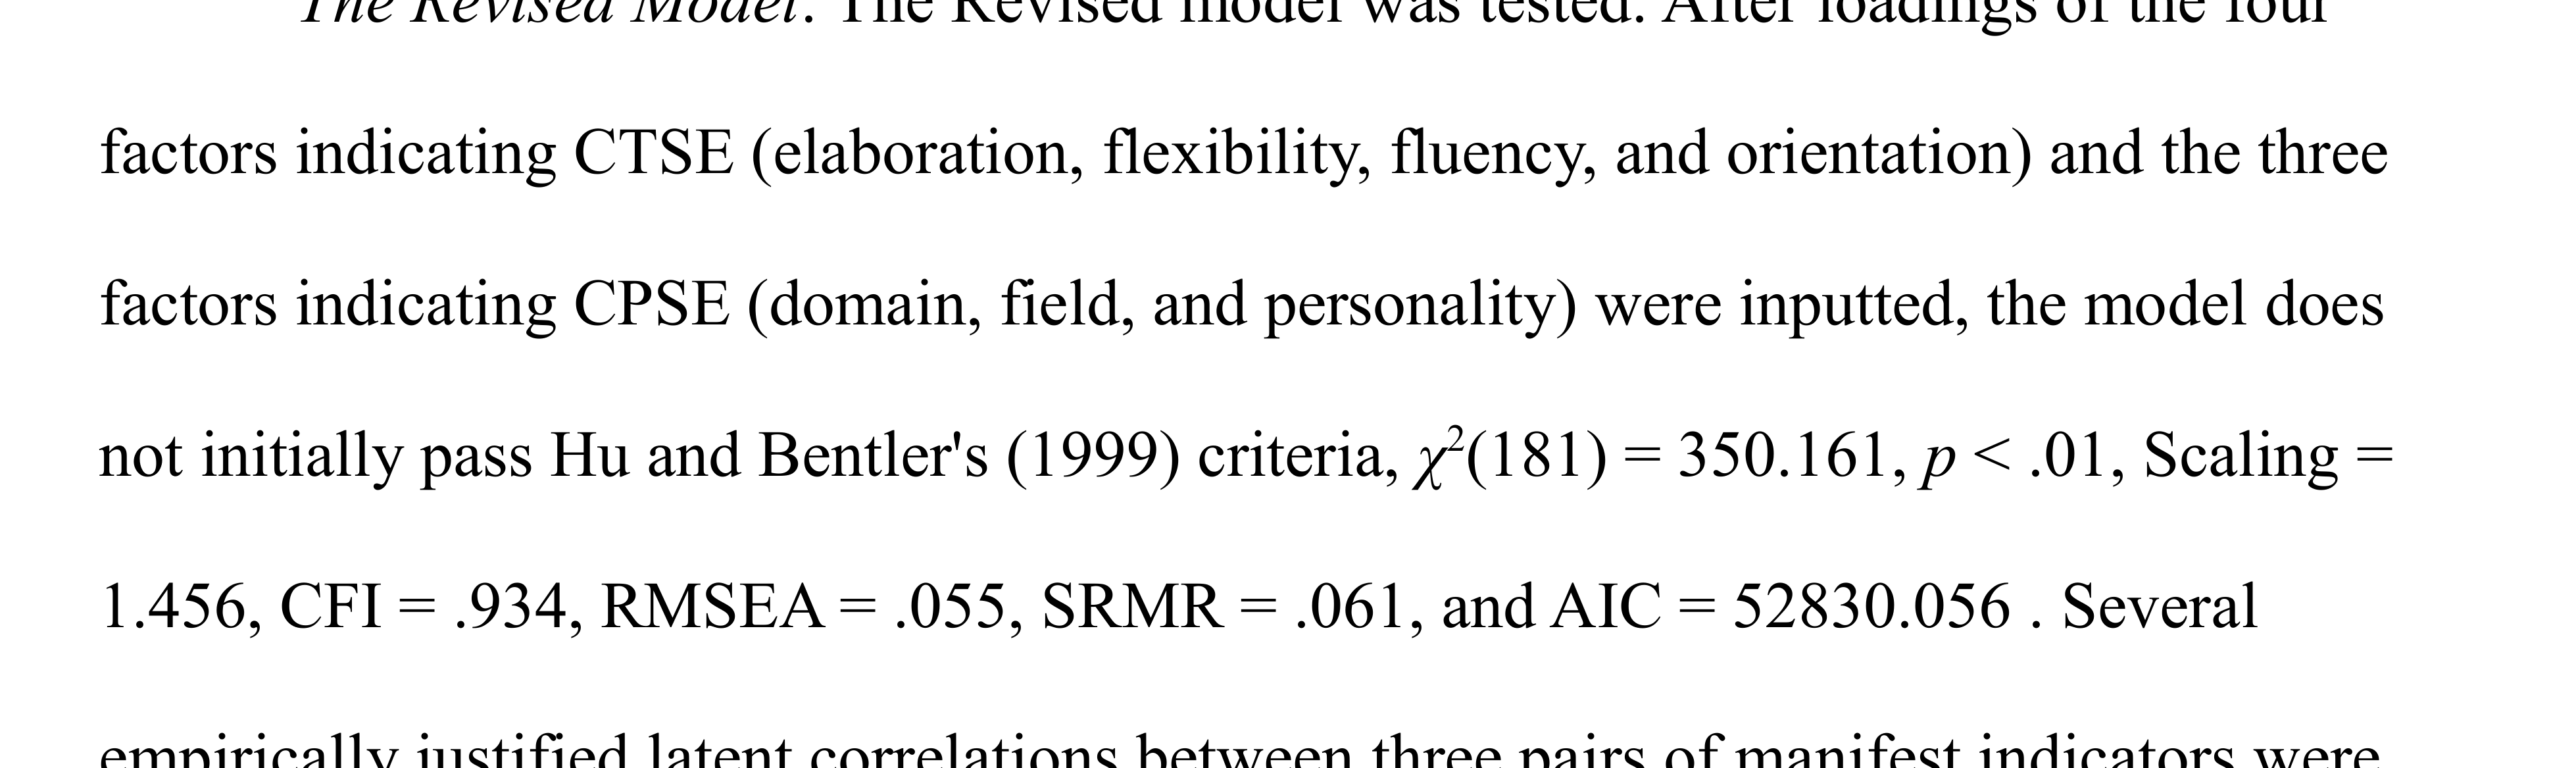
\includegraphics[width=\textwidth]{figures/initial_fit.png}
\caption{Printed page~129. The initial model and the word
``orientation'' in the sentence that names the four thinking factors.}
\label{fig:initial}
\end{figure}

\section{What we replicated}
\label{sec:replicated}

This section answers which printed claims agree with a direct fit to
Table~3.2.
Table~\ref{tab:compare} is that comparison.
``Match'' means the same degrees of freedom, the same rounded index, or
the same ordering.
``Close'' means a gap on the order of the third printed decimal, or a
chi-square gap of a few points on a difference.
``Partial'' means one piece of the claim holds and another does not.
``No match'' means a different number after the checks in
Section~\ref{sec:tried}.

\begin{table}[ht]
\centering
\small
\begin{tabular}{@{}p{0.28\textwidth}p{0.24\textwidth}p{0.26\textwidth}p{0.12\textwidth}@{}}
\toprule
Claim & Published & Ours & Verdict \\
\midrule
Degrees of freedom, nine Appendix~J models &
The nine values in the caption &
The same nine numbers &
match \\
Refined model, SRMR &
\(.057\) &
\(.0578\) &
close \\
Refined model, CFI and RMSEA &
\(.954\) and \(.046\) &
\(.939\) and \(.072\), maximum likelihood &
partial \\
Scaled difference for three residual correlations &
\(\chi^2(3)=52.457\) &
\(52.457\) from the printed inputs &
match \\
Maximum-likelihood difference for those correlations &
Unscaled difference \(77.41\) &
\(75.08\) on \(3\) df &
close \\
General factor is the worse model &
CFI \(.945\), higher AIC &
CFI \(.930\), higher chi-square &
match \\
Negative scaled difference &
\(\chi^2(2)=-21.803\) &
\(+4.02\) on \(1\) df from the same algebra &
no match \\
Parsimony order &
Revised, then implied structure, implied indicators, all, held &
The same order &
match \\
AIC gap, revised against all indicators &
\(235.09\) &
\(234.12\) &
match \\
AIC gap, revised against implied structure &
\(64.47\) &
\(34.38\) &
no match \\
Implied-structure chi-square, unscaled &
\(526.884\times 1.357=714.98\) &
\(715.13\) &
match \\
BCSE with CTSE and with CPSE &
\(.53\) and \(.69\) &
\(.529\) and \(.685\) &
close \\
Openness with CTSE and with CPSE &
\(.45\) and \(.53\) &
\(.435\) and \(.523\) &
close \\
Kaiser--Meyer--Olkin index &
\(.93\) &
\(.925\) on all \(37\) columns &
match \\
\bottomrule
\end{tabular}
\caption{Printed claims against the fits in
\texttt{simulation/out/comparison.csv}.
BCSE is Beghetto's creative self-efficacy measure.
AIC is the Akaike information criterion.
The nine degrees of freedom belong, in order, to the initial model,
the refined model, the general-factor model, the span model, the
revised model with saturated correlates, the all-indicator model, the
held model, the implied-structure model, and the implied-indicators
model.}
\label{tab:compare}
\end{table}

The degrees of freedom fix the specification.
For \(21\) revised indicators the initial model has \(231\) sample
moments and \(50\) free parameters, so the degrees of freedom are
\(181\).
Three residual covariances bring that to \(178\).
Freeing the two second-order marker loadings and fixing the two
second-order variances and their covariance at \(1\) changes the count
by one, to \(179\).
Those are the printed degrees of freedom.
The same count holds for the six larger models, including the
all-indicator model at \(536\) and the held model at \(311\).

The standardized root mean square residual is computed from the
correlation residuals of the maximum-likelihood point estimates.
It does not use the robust scaling factor.
The initial model gives \(.0612\) against the printed \(.061\).
The all-indicator model gives \(.0621\) against \(.062\).
The held model gives \(.0599\) against \(.060\).
The refined model gives \(.0578\) against \(.057\).
Figure~\ref{fig:refined} is the refined line.

\begin{figure}[ht]
\centering
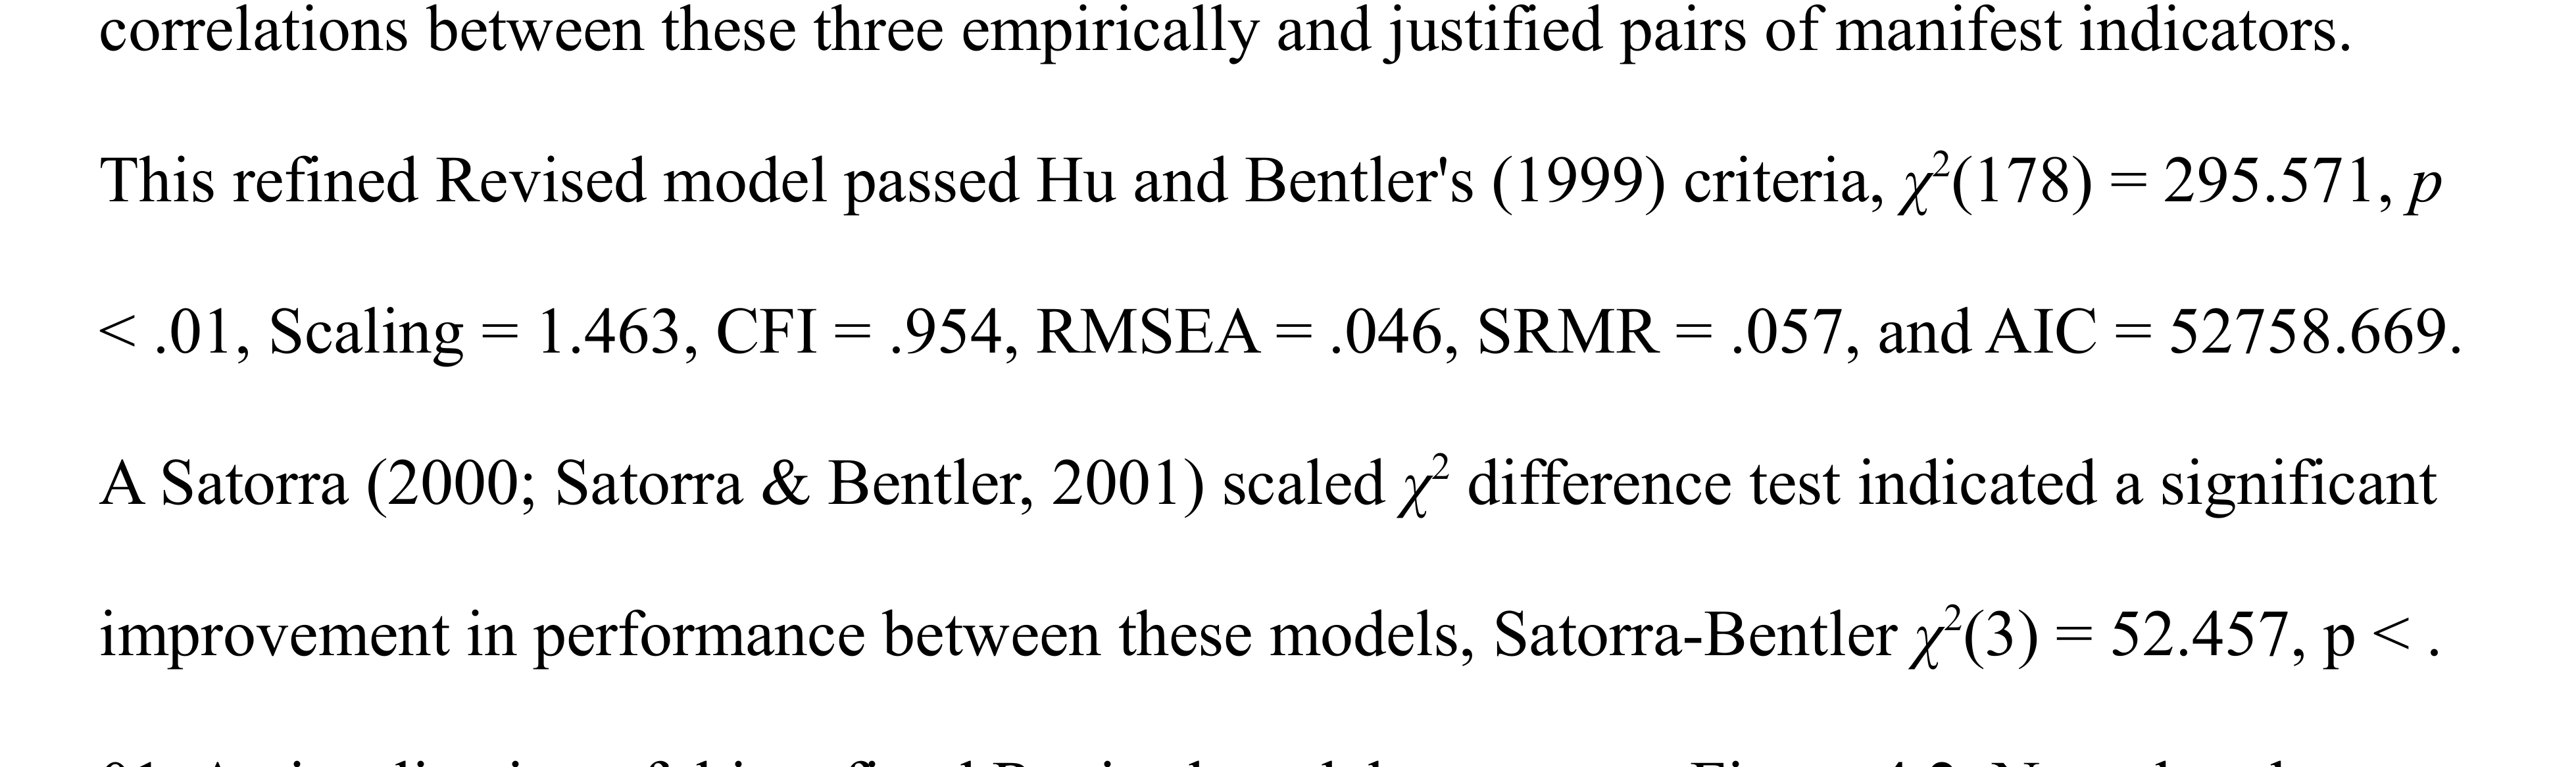
\includegraphics[width=\textwidth]{figures/refined_fit.png}
\caption{Printed page~130. The refined model and the scaled difference
of \(52.457\) on \(3\) degrees of freedom.}
\label{fig:refined}
\end{figure}

The scaled difference uses the printed chi-squares and the printed
scaling factors.
With \(T\) the scaled chi-square, \(d\) the degrees of freedom, and \(c\)
the scaling factor,
\[
  c_d=\frac{d_0 c_0-d_1 c_1}{d_0-d_1},\qquad
  \frac{T_0-T_1}{c_d}.
\]
For the initial model against the refined model this is
\(52.457\), the printed value.
The function is
\srcat{simulation/fit_models.R}{417}.
The maximum-likelihood chi-square difference on our fits is \(75.08\)
on \(3\) degrees of freedom.
The difference of the two unscaled products,
\(350.161\times 1.456-295.571\times 1.463\), is \(77.41\).
The two differences sit \(2.3\) apart.

Mplus prints a scaled chi-square under MLR and a scaling factor such
that the product is the ordinary maximum-likelihood chi-square.
For the implied-structure model that product is \(714.98\), and our
chi-square is \(715.13\).
For the implied-indicators model the product is \(780.21\) and our
chi-square is \(778.45\).
For the revised model the product is \(432.42\) and our chi-square is
\(450.69\).
The comparative fit index and the root mean square error of
approximation printed for the revised model are computed from the
scaled chi-square.
Our maximum-likelihood versions are \(.939\) and \(.072\).
They do not pass the cuts \(\mathrm{CFI}>.95\) and
\(\mathrm{RMSEA}<.06\).
The printed robust indices do pass those cuts.
The standardized residual index, which does not use that scaling,
passes \(\mathrm{SRMR}<.09\) on both sides.

The Akaike information criterion is on different numeric levels because
it depends on the sample size and on \(\log|\Sigma|\), and the printed
standard deviations are rounded to one decimal.
On the models that use the same observed variables, the order is the
printed order.
The revised model with saturated correlates has the lowest value, then
the implied-structure model, the implied-indicators model, the
all-indicator model, and the held model.
The gap against the all-indicator model is \(234.12\) against \(235.09\).
The gap against the implied-structure model is \(34.38\) against the
printed \(64.47\).
That second gap is the chi-square gap between those two models, shifted
by two points for the extra parameter.
Our chi-square gap is about \(36\), and the gap of the unscaled printed
chi-squares is about \(67\).

Beghetto's measure correlates with creative thinking self-efficacy at
\(.529\) against \(.53\), and with creative performance self-efficacy at
\(.685\) against \(.69\).
Openness correlates with those two factors at \(.435\) against \(.45\)
and \(.523\) against \(.53\).
Across the \(55\) off-diagonal entries in Table~4.1, the mean absolute
gap is \(0.0065\) and one entry exceeds \(0.02\): openness with
flexibility, \(.390\) against \(.41\).
The file is \src{simulation/out/table41_gaps.csv}.

The Kaiser--Meyer--Olkin index on all \(37\) columns of Table~3.2 is
\(0.925\), which rounds to the printed \(.93\).
The index on the creative-thinking and creative-performance items alone
is \(0.935\).
The function is \srcat{simulation/fit_models.R}{42}.

The first-order composite reliabilities use the square of the sum of
the standardized loadings in the numerator.
On the refined model that quantity is \(0.596\) for fluency, \(0.910\)
for domain, \(0.842\) for field, and \(0.890\) for personality, against
the Table~4.2 entries \(0.60\), \(0.91\), \(0.84\), and \(0.89\).
Elaboration is \(0.771\) against \(0.78\).
Flexibility is \(0.882\) against \(0.93\), and originality is \(0.935\)
against \(0.88\).
The ratio written on printed page~110, with the sum of squared loadings
in the numerator, gives fluency \(0.356\) and does not match those
cells.
Both columns are in \src{simulation/out/composite_validity.csv}.

\section{What gave trouble, and how it was resolved}
\label{sec:tried}

This section answers where a first reading disagreed with a printed
number, and which change removed the disagreement.
The disagreements that remain are in Section~\ref{sec:open}.

The sample size and the likelihood were the first check.
Table~3.2 prints \(n=296\).
Table~4.1 prints \(n=308\).
The text also says \(297\) people completed every item.
A grid of \(296\), \(297\), and \(308\), each with the Wishart
likelihood and with the normal likelihood, is in
\src{simulation/out/n_likelihood_grid.csv}.
The Wishart fit at \(296\) is the closest of those six to
\(350.161\times 1.456\), the unscaled target for the initial model.
The remaining gap there is \(15.9\) chi-square points.
Changing the sample size multiplies the chi-square.
It does not remove that gap.
The same Wishart fit at \(296\) does land on the implied-structure
target, so the multiplier is not a single global error.

The robust scaling was the second check.
Dividing our refined chi-square by the printed scaling factor
\(1.463\) produces \(308.1\), against the printed scaled value
\(295.571\).
The comparative fit index and the root mean square error of
approximation move with that scaled value, and with the baseline
model's own scaling factor, which is not printed.
We therefore compare the ordinary maximum-likelihood chi-square with
the product of the printed scaled chi-square and the printed scaling
factor, and we compare the standardized residual index directly.

The optimizer was the third check.
lavaan~\cite{rosseel2012} with \texttt{nlminb} and with BFGS agree to
about \(0.07\) chi-square points on the initial, refined, general-factor,
and span models.
OpenMx~\cite{neale2016} with SLSQP and with CSOLNP agree with each
other to \(10^{-5}\).
OpenMx multiplies the fit function by \(N\).
lavaan's Wishart likelihood multiplies it by \(N-1\).
Rescaling the lavaan initial chi-square by \(296/295\) gives \(527.56\).
The OpenMx value is \(527.52\).
The refined and general-factor models show the same relationship.
The file is \src{simulation/out/openmx_fits.csv}.
The optimizer is not the source of the gap with the printed robust
chi-square.

The saturated-correlate models needed a separate start.
lavaan's default starts make the initial model-implied matrix fail to
be positive definite once unused items are given free covariances with
every other item.
Starting those covariances at zero, and starting residual variances
from the sample variances, lets the models converge.
The iteration limit in \srcat{simulation/fit_models.R}{311} is \(3000\).
The revised model with saturated correlates then has chi-square
\(678.87\) and \(326\) degrees of freedom, against \(678.86\) and \(326\)
for the same focal model without the extra items.
Adding a saturated item does not change the degrees of freedom or,
here, the chi-square.
That is the pattern in the printed pair \(514.150\) and \(514.108\) as
well.
lavaan warns that the residual covariance matrix is not positive
definite for the four models that carry those extra covariances.
The implied-structure model carries that warning and still matches its
unscaled target, so the warning alone does not identify the revised
model's chi-square gap.

The general-factor difference test was checked as algebra before it was
treated as a discrepancy.
The printed degrees of freedom are \(179\) and \(178\), so a nested
comparison has \(1\) degree of freedom.
The code frees the two marker loadings and fixes three second-order
moments, which is the same net change of one parameter.
The algebra that returns \(52.457\) for the three residual correlations
returns \(+4.02\) for this comparison.
The printed line is \(\chi^2(2)=-21.803\).
Figure~\ref{fig:general} is that line.
Our maximum-likelihood difference is \(+40.73\) on \(1\) degree of
freedom, against the unscaled printed difference \(42.94\).
The general-factor model fits worse on both accounts.
The negative two-degree-of-freedom figure is the cell that remains.

\begin{figure}[ht]
\centering
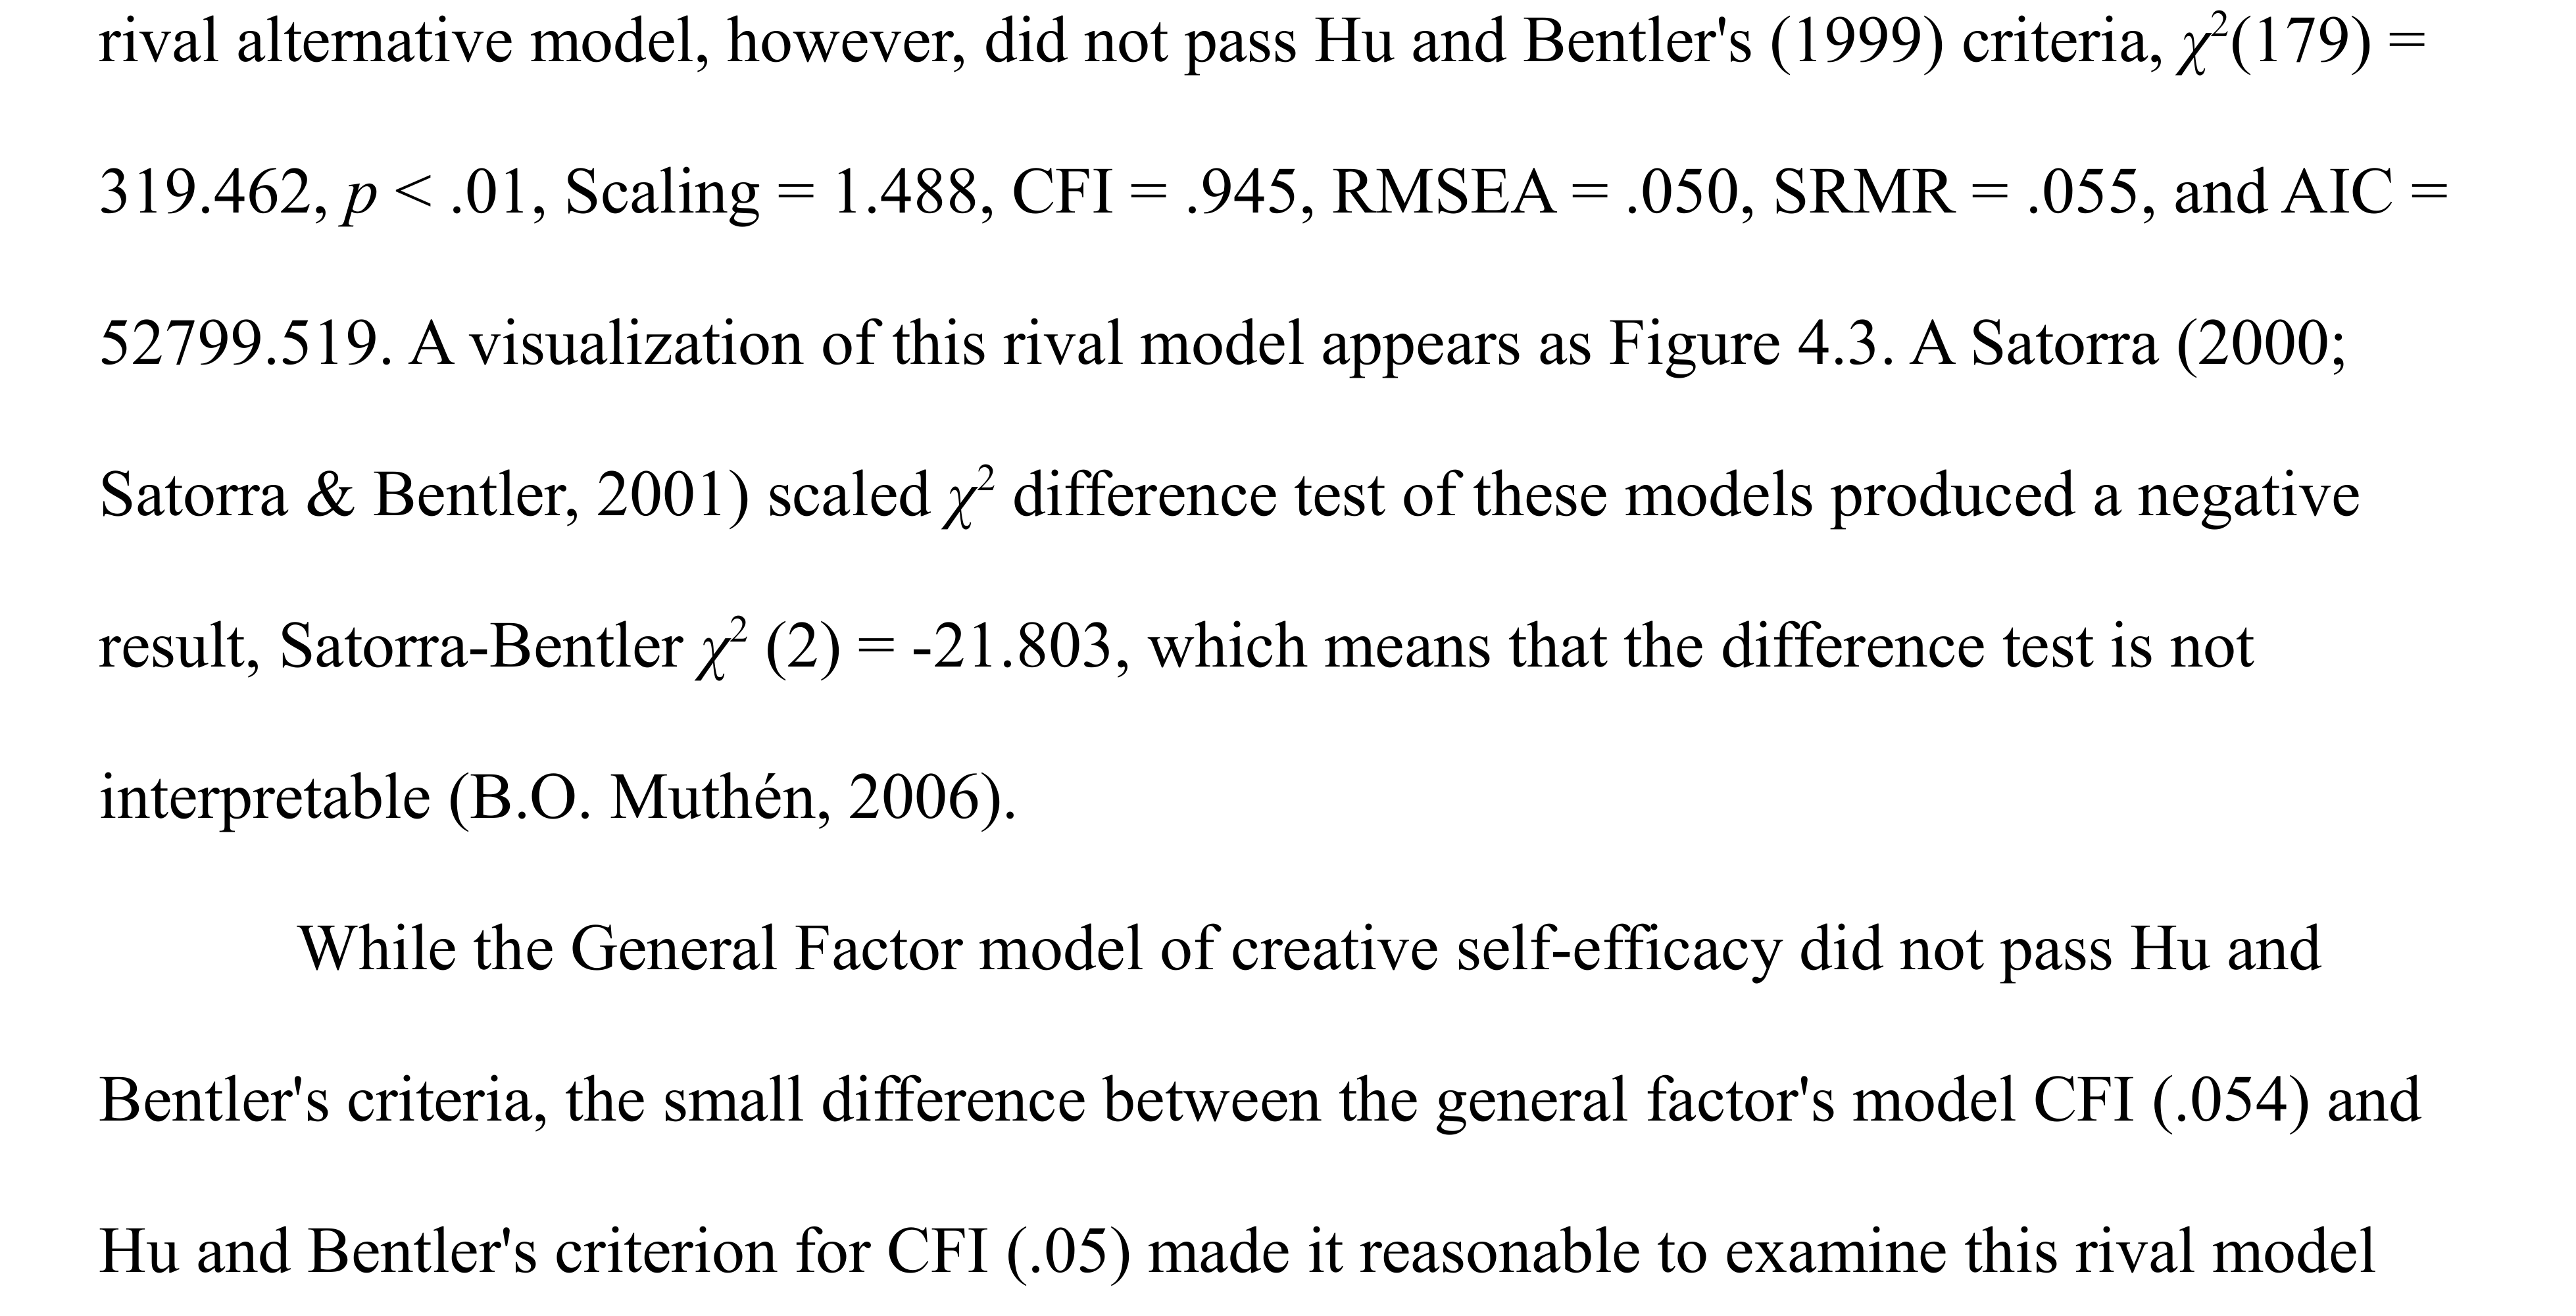
\includegraphics[width=\textwidth]{figures/general_factor.png}
\caption{Printed page~131. The general-factor fit, the negative
difference, and the parenthetical comparative fit index.}
\label{fig:general}
\end{figure}

The parenthetical on that page says the general-factor comparative fit
index is \(.054\) and the criterion is \(.05\).
The fit line two paragraphs above prints \(\mathrm{CFI}=.945\).
The criterion stated for that index earlier in the dissertation is
\(.95\).
The comparison in Table~\ref{tab:compare} uses the fit line.

The word on printed page~129 for the fourth thinking factor is
``orientation.''
Appendix~J names the factor with the originality items
\texttt{CTORIG1} through \texttt{CTORIG4}.
The model we fit uses those items.
Figure~\ref{fig:initial} shows both the word and the fit line.

\section{What we did ourselves, and what we took from others}
\label{sec:ours}

This section answers which pieces are ours and which pieces are taken
from the dissertation.
The dissertation contributes the inventories, the factor structure, the
rival models, and the printed tables.
We contribute the covariance matrix read from Table~3.2, the
maximum-likelihood fits, the OpenMx check, and the comparison.

The three residual covariances are the ones named in the text and
written in Appendix~J: elaboration items~4 and~5, domain items~1 and~4,
and personality item~2 with field item~2.
On the initial model, those three pairs are among the larger
modification indices for residual covariances.
The largest modification index is a factor residual covariance, which
the dissertation does not free.
We did not add it.

No number in the comparison is taken from a later paper.
The composite-reliability formula with the square of the sum of the
loadings is the usual one.
The dissertation's page~110 writes the sum of squared loadings in the
numerator.
Both are computed in the output file named above.
Table~4.2's fluency, domain, field, and personality entries agree with
the usual formula.

\section{Assumptions}
\label{sec:assumptions}

Each subsection is a choice the dissertation does not settle and that
the fits require.

\subsection{The printed matrix is one complete-data covariance matrix}

Table~3.2 prints a correlation, a mean, and a standard deviation for
each of \(37\) columns, at \(n=296\).
Eleven of the \(308\) people who started the instrument left at least
one item blank, and \(297\) people completed every item.
The dissertation estimates the models by full-information maximum
likelihood on the raw file.
We treat the printed correlations and standard deviations as the
covariance matrix of one complete sample of size \(296\).
The standard deviations enter only the scale of the covariance matrix.
A confirmatory factor model with a marker loading fixed at \(1\) is
invariant to rescaling each observed variable, so the chi-square does
not depend on those standard deviations.
It does depend on the correlations.
The correlations are printed to two decimals.
Figure~\ref{fig:table32} shows the fluency item whose standard
deviation is \(52.3\), and a minus sign on a later row.

\begin{figure}[ht]
\centering
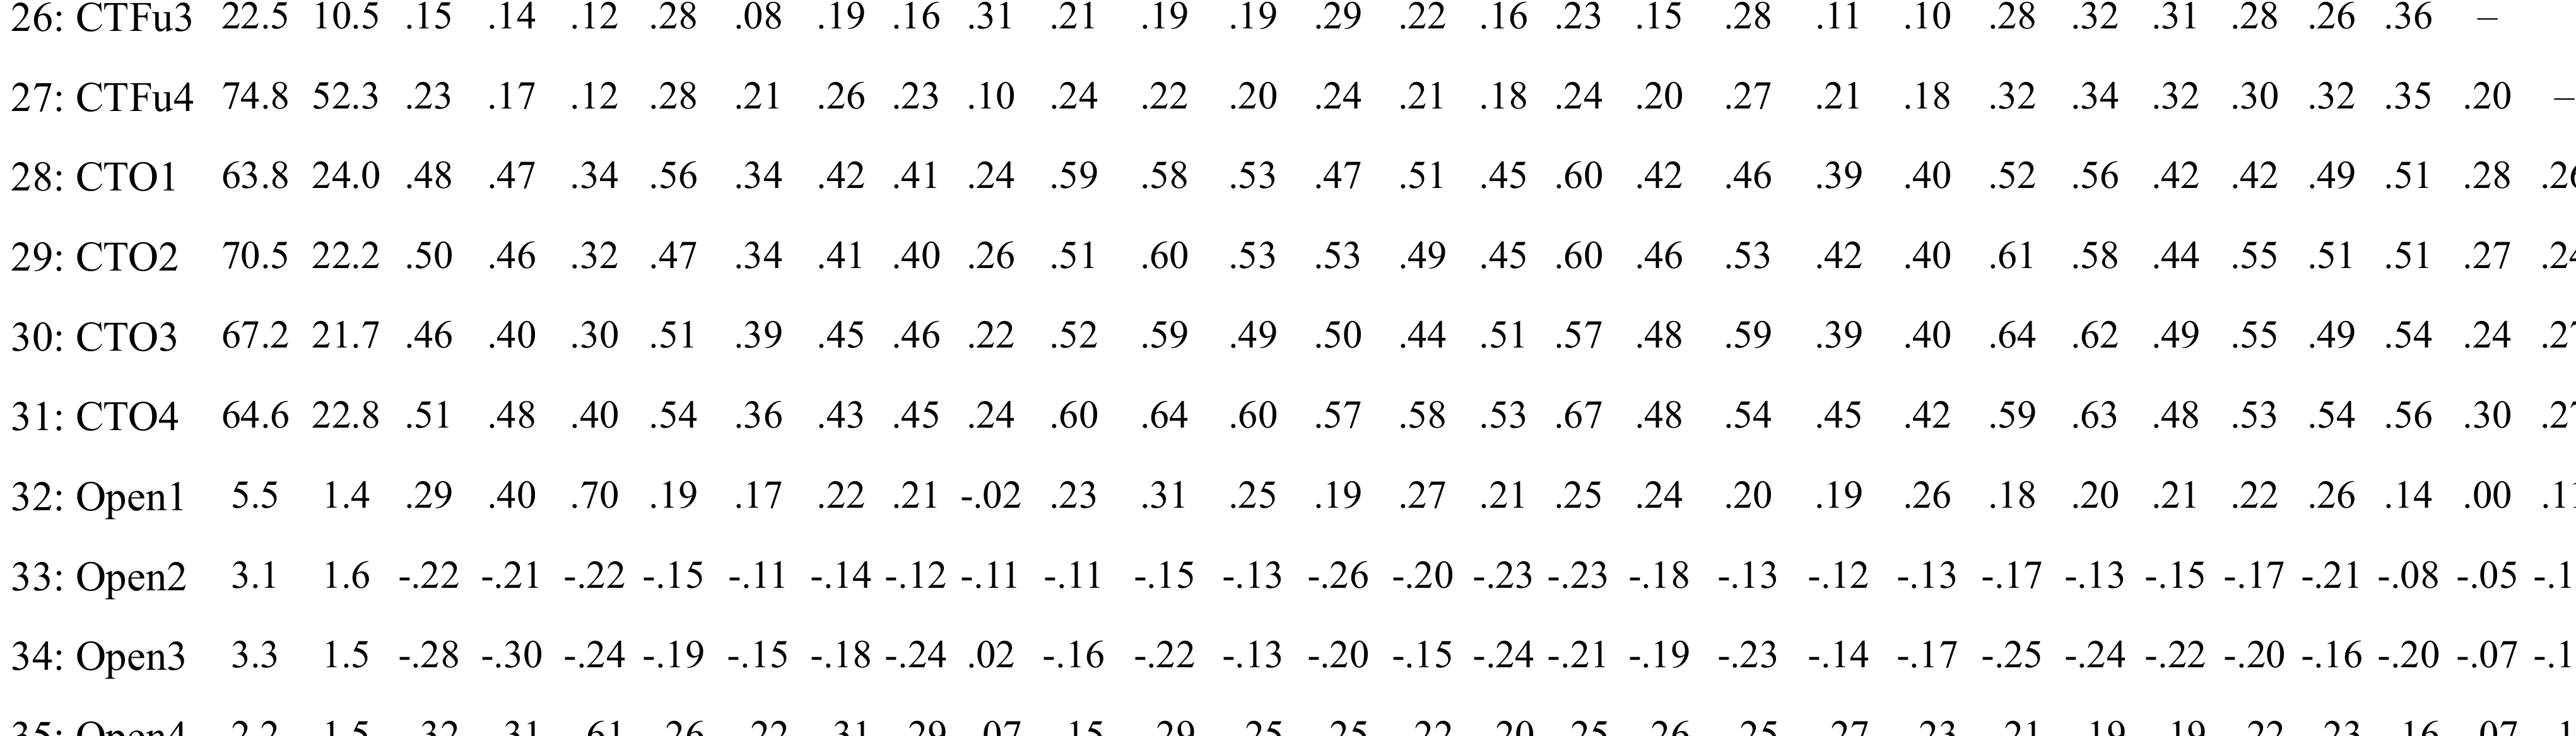
\includegraphics[width=\textwidth]{figures/table32_ctfu4.png}
\caption{Printed page~95. The row for fluency item~4, with standard
deviation \(52.3\), and minus signs in the rows below it.}
\label{fig:table32}
\end{figure}

\subsection{Row labels map onto the Appendix~J names in printed order}

The table's note gives the block order: Beghetto's three items, four
domain items, four field items, four personality items, elaboration,
flexibility, fluency, originality, four openness items, sex, and age.
Elaboration begins at item~2, so \texttt{CTELAB1} is not in the table.
The tenth row is labeled \texttt{CPFI} and sits between field items~2
and~4.
We read it as field item~3, \texttt{CPFIEL3}.
Both the revised model and the implied-structure model use that item
as an indicator.
The implied-structure chi-square matches its unscaled target under this
reading.

\subsection{The Wishart likelihood at \(n=296\)}

lavaan can multiply the fit function by \(N-1\) or by \(N\).
Mplus~5.2's ordinary maximum-likelihood chi-square is the fit function
times a sample-size factor as well.
We use the Wishart choice, \(N-1\), at the sample size printed on
Table~3.2.
Section~\ref{sec:tried} records the grid.
Latent means are fixed at zero and observed intercepts are free, so the
mean structure is saturated and does not add to the chi-square.

\subsection{Marker identification, with the general-factor loadings free}

Appendix~J fixes the first loading of each first-order factor at \(1\).
In the general-factor model the first loading of each second-order
factor is free, and the two factor variances and their covariance are
fixed at \(1\).
lavaan will put a loading of \(1\) back on the first indicator if the
syntax names that indicator twice.
The syntax uses a single free parameter on each of those two loadings.
The estimates are free in
\src{simulation/out/general_second_order_loadings.csv}.

\subsection{Openness items~2, 3, and~4 keep the printed signs}

Those three columns correlate negatively with the creative
self-efficacy items.
Openness item~1 correlates positively with them.
We do not reverse the three columns before the fit.
Their loadings start negative so that the first model-implied matrix
can be positive definite.
The signs of the loadings are estimated, not fixed.

\section{Ambiguities that were resolved}
\label{sec:resolved}

This section answers which printed details were ambiguous and which
file now settles them.

The tenth row of Table~3.2 is labeled \texttt{CPFI}.
The resolution is the order in the table note together with the
implied-structure chi-square.
The script that reads the text layer is
\srcat{simulation/parse_table32.py}{1}, and the matrix is
\src{simulation/table32.csv}.
Regenerating the matrix from the PDF is
\texttt{python3 formalization/abbott-ctse/simulation/parse\_table32.py}
with the PDF path.
The committed matrix matches that reading.

The sentence on printed page~110 writes composite validity as
\(\sum\lambda^2/(\sum\lambda^2+\sum\varepsilon)\).
The Table~4.2 entries for fluency, domain, field, and personality match
the square of the sum of the standardized loadings instead.
The output file records both.
The command is \texttt{Rscript fit\_models.R out} from
\texttt{formalization/abbott-ctse/simulation}.

The saturated-correlate syntax is the block of \texttt{WITH} statements
in Appendix~J.
Each unused item is given a free covariance with every other observed
variable, once.
The function is \srcat{simulation/fit_models.R}{148}.
After the starts in Section~\ref{sec:tried}, those models converge, and
their degrees of freedom match the printed degrees of freedom.

\section{What remains unresolved}
\label{sec:open}

This section answers which printed numbers are still apart from the
fits, and which checks did not close the gap.

The refined model's ordinary chi-square is \(450.69\) against the
unscaled target \(432.42\).
The initial model is \(525.77\) against \(509.83\).
The span model is \(678.86\) against \(648.34\).
The same matrix produces \(715.13\) against \(714.98\) for the
implied-structure model, and \(778.45\) against \(780.21\) for the
implied-indicators model.
The gap is therefore not a single multiplier on every model.
Full-information maximum likelihood on the raw file, with eleven
partially observed people, is the check that would use a different
matrix for each pattern of missing items.
The file named in Appendix~J, \texttt{CohortsTwo.dat}, is the file that
would settle it.
Two-decimal rounding of the correlations is a second open contributor.
A perturbation of each correlation by up to half a hundredth did not
return a stable band: the perturbed matrices did not converge under the
same starts.
That attempt is not used as a tolerance.

The comparative fit index and the root mean square error of
approximation of the refined model remain the robust versions.
Recomputing them requires the baseline model's scaling factor as well
as the focal one.
The printed focal scaling factor is \(1.463\).
The baseline factor is not printed.

The negative difference is the other cell.
The inputs are the printed chi-squares \(319.462\) and \(295.571\), the
scaling factors \(1.488\) and \(1.463\), and the degrees of freedom
\(179\) and \(178\).
The algebra that reproduces \(52.457\) gives \(+4.02\) on \(1\) degree of
freedom.
The printed line is \(-21.803\) on \(2\) degrees of freedom.
The models are not a pair in which one set of free parameters is a
subset of the other in a single parameterization: the general-factor
model frees the marker loadings and fixes the second-order moments.
A raw-data run in Mplus~5.2, with the scaling factors and the
difference test written to the output, is the check.

The fraction of correlations greater than \(.30\) is printed as \(.66\).
On all \(37\) columns the fraction of absolute correlations above \(.30\)
is \(.544\).
On the creative-thinking and creative-performance items it is \(.817\).
Within the factor blocks it is \(.843\).
None of those readings is \(.66\).
The Kaiser--Meyer--Olkin index from the same matrix does round to
\(.93\).

The Akaike gap against the implied-structure model is \(34.38\) against
\(64.47\).
That gap moves with the revised model's chi-square.
It is the same open question as the chi-square level, not a separate
one.

Smaller differences, kept out of the verdicts above, are these.
The refined standardized residual rounds to \(.058\) against the printed
\(.057\).
The general-factor residual rounds to \(.056\) against \(.055\).
The implied-structure residual rounds to \(.050\) against \(.049\).
The span residual rounds to \(.059\) against \(.058\).
Beghetto's correlation with creative performance self-efficacy rounds
to \(.68\) or \(.69\) depending on the rounding rule; the printed value
is \(.69\) and ours is \(.685\).
These are the third-decimal gaps.
They are not, by themselves, a failure of the degrees of freedom or of
the parsimony order.
Figure~\ref{fig:table41} is the correlation table.

\begin{figure}[ht]
\centering
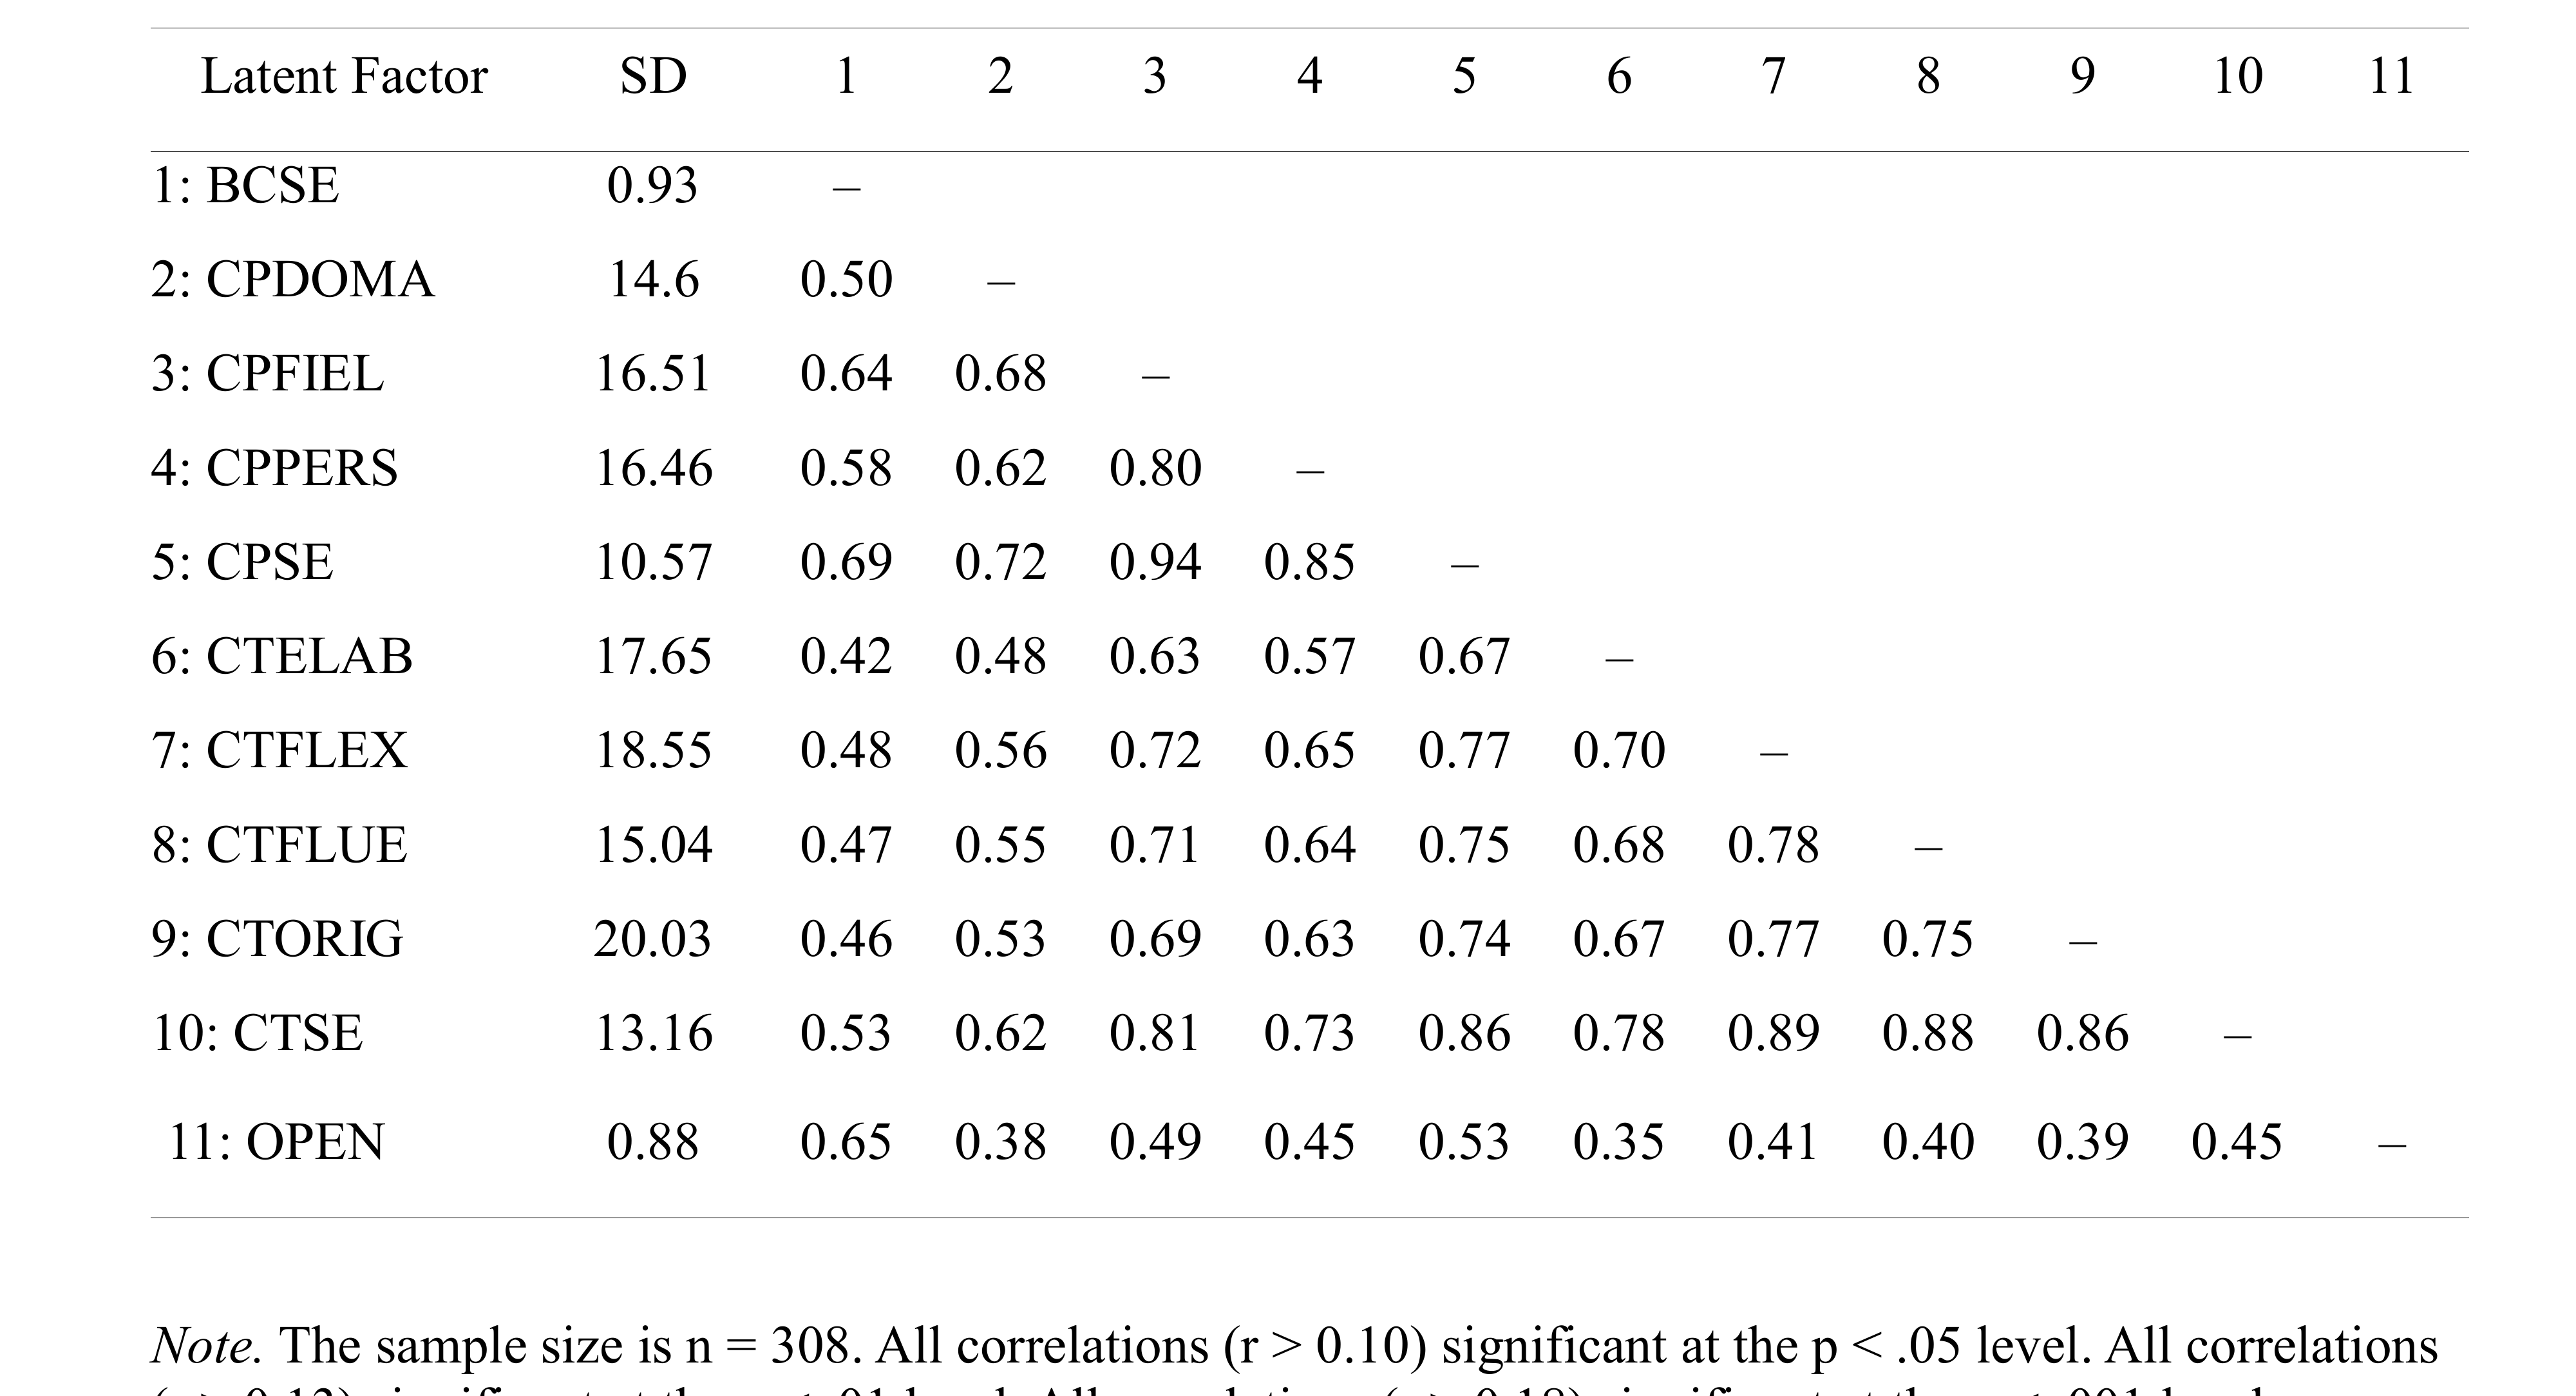
\includegraphics[width=\textwidth]{figures/table41.png}
\caption{Printed page~135. Latent correlations for the revised model
with Beghetto's measure and openness.}
\label{fig:table41}
\end{figure}

\section{Code and source availability}
\label{sec:availability}

This section answers where the dissertation and the analysis code were
sought.
The dated rows are the ledger in
\src{simulation/out/code_search.md}.

\begin{center}
\footnotesize
\begin{tabular}{@{}p{0.42\textwidth}p{0.16\textwidth}p{0.34\textwidth}@{}}
\toprule
Place & Date & Result \\
\midrule
UNL PDF via Wayback \texttt{20261004155053} &
2026-10-29 &
Obtained. sha256 \texttt{a3c381d6\ldots}\\
Direct curl of the UNL download URL &
2026-10-29 &
HTTP 403, bot check \\
ProQuest docview \texttt{305217740} &
2026-10-29 &
HTML page. PDF bytes not saved \\
Ledger copy of the same dissertation &
2026-10-29 &
Different sha256, file not in this fit \\
Appendix~J path \texttt{CohortsTwo.dat} &
2026-10-29 &
Local path only. Not obtained \\
GitHub, GitLab, OSF, Zenodo &
2026-10-29 &
No analysis repository and no raw file \\
Mplus 5.2 &
2026-10-29 &
Named in Appendix~J. Not installed \\
\bottomrule
\end{tabular}
\end{center}

The PDF used for the crops and for the matrix has sha256
\sha{a3c381d6f6295e917806834364b7f55fc35684b3db53174a53c3564feab4d70a}.
It is a \(283\)-page file whose producer line is Prince~15.4.1 and whose
creation date is 30~August~2026.
The literature ledger records a different hash,
\sha{d39a696d20d6df6d9467a8906e67c40f336c3856ac74637f8db6629ca9fcc9d2},
for a file of the same page count.
The fits and the crops in this note are from the file we obtained.

R~\cite{rcore} is version \(4.3.3\).
It is the program named, in the \(2009\) citation, as the general tool
for the quantitative work.
lavaan~\cite{rosseel2012} is version \(0.6.17\), from
\url{https://CRAN.R-project.org/package=lavaan}.
It fits the mean and covariance model that Appendix~J specifies,
because Mplus~5.2 is not installed here.
OpenMx~\cite{neale2016} is version \(2.21.11\), from
\url{https://CRAN.R-project.org/package=OpenMx}.
It is the second optimizer.
The versions are the \texttt{sessionInfo} record in
\src{simulation/out/sessionInfo.txt}.

\section{Next steps}

The raw file \texttt{CohortsTwo.dat}, or an Mplus~5.2 output that
prints the unscaled chi-square, the baseline scaling factor, and the
difference test, is the check that separates the revised model's
chi-square level from the robust scaling and from full-information
maximum likelihood.
The same file would recompute the fraction of correlations above
\(.30\).
The ProQuest file whose hash is recorded in the literature ledger would
show whether any printed entry in Table~3.2 differs from the file used
here.
The interview phase remains outside this comparison.
It would be a reading of the transcripts, not a refit of Table~3.2.

\section{Artifacts}
\label{app:artifacts}

\begin{itemize}
\item Matrix.
File \src{simulation/table32.csv}.
Command: \texttt{python3}~\src{simulation/parse\_table32.py}
with the PDF.
\item Fits.
File \src{simulation/out/comparison.csv},
\src{simulation/out/lavaan\_fits.csv},
\src{simulation/out/openmx\_fits.csv}.
Command, from \texttt{formalization/abbott-ctse/simulation}:
\texttt{Rscript}~\srcat{simulation/fit_models.R}{311}~\texttt{out}.
\item Sample-size grid.
File \src{simulation/out/n\_likelihood\_grid.csv}.
Same command.
\item Scaled-difference algebra.
File \src{simulation/out/satorra\_printed.csv}.
Function \srcat{simulation/fit_models.R}{417}.
\item Latent correlations.
File \src{simulation/out/table41\_gaps.csv}.
\item Composite reliability.
File \src{simulation/out/composite\_validity.csv}.
\item Matrix indices.
File \src{simulation/out/matrix\_checks.csv}.
Function \srcat{simulation/fit_models.R}{42}.
\item Rounding draws.
File \src{simulation/out/rounding\_band.csv}.
Three draws, seed \(20100501\). Each chi-square is missing because the perturbed matrix did not converge.
\item OpenMx.
Function \srcat{simulation/fit_models.R}{602}.
File \src{simulation/out/openmx\_fits.csv}.
\item Availability ledger.
File \src{simulation/out/code\_search.md}.
\item Page crops.
Directory \src{paper/figures}.
Command, from the repository root:
\texttt{python3}~\src{paper/figures/crop\_pages.py}.
\end{itemize}

The dissertation PDF is local and is not in git.

\begin{thebibliography}{9}

\bibitem{rcore}
R Core Team.
\emph{R: A Language and Environment for Statistical Computing}.
R Foundation for Statistical Computing, Vienna, Austria, 2024.
\url{https://www.R-project.org/}.

\bibitem{rosseel2012}
Yves Rosseel.
lavaan: An R package for structural equation modeling.
\emph{Journal of Statistical Software} 48(2) (2012), 1--36.
\href{https://doi.org/10.18637/jss.v048.i02}{10.18637/jss.v048.i02}.
Package page: \url{https://CRAN.R-project.org/package=lavaan}.

\bibitem{neale2016}
Michael C.~Neale, Michael D.~Hunter, Joshua N.~Pritikin, Mahsa Zahery,
Timothy R.~Brick, Robert M.~Kirkpatrick, Ryne Estabrook,
Timothy C.~Bates, Hermine H.~Maes, and Steven M.~Boker.
OpenMx 2.0: Extended structural equation and statistical modeling.
\emph{Psychometrika} 81(2) (2016), 535--549.
\href{https://doi.org/10.1007/s11336-014-9435-8}{10.1007/s11336-014-9435-8}.
Package page: \url{https://CRAN.R-project.org/package=OpenMx}.

\end{thebibliography}

\end{document}
